\section{Problema 4}
Suponga que se quiere estimar el promedio diario de producción $\mu$ de un producto farmacéutico con un error de estimación menor que 3 toneladas con probabilidad de $0.95$. Además, se sabe que la amplitud de la producción es aproximadamente 120 toneladas. Calcule el tamaño muestral de forma que se tenga cierta seguridad (con un coeficiente de alrededor de $0.95$ ) de que la estimación se encuentra a no más de 3 toneladas del verdadero promedio diario de producción (Para poder realizar dicho procedimiento, incluya las suposiciones pertinentes). (Valor 25 puntos).
\begin{solution}
Empezamos analizando los datos proporcionados: 
\begin{enumerate}
    \item Ya que 95\% de las medias muestras no estarán a más de $2\sigma_{\overline{Y}}$ del $\mu$ en muestreo repetido, es decir que estamos pidiendo que $2\sigma_{\overline{Y}}$ sea igual a 3 toneladas. Gráficamente: 
    \begin{center}
        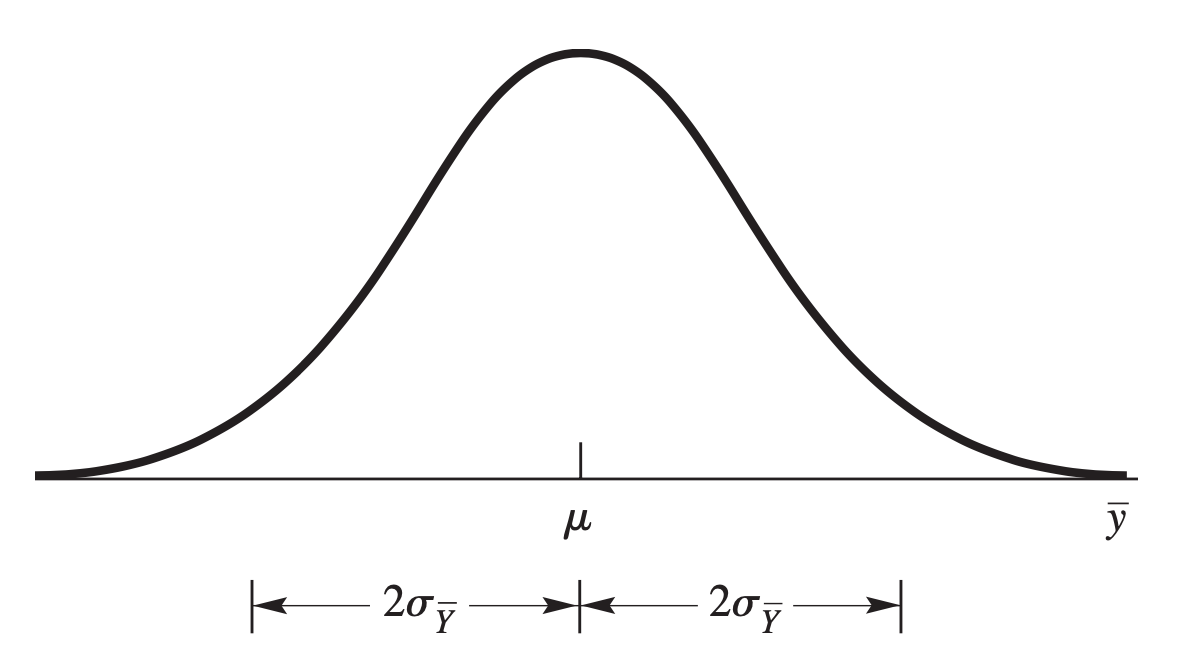
\includegraphics[scale=0.2]{Images/Problema4-1.png}
    \end{center}
    Es decir, que lo que nos están pidiendo es: 
    $$\frac{2\sigma}{\sqrt{n}}=
    3\implies n=\frac{4\sigma^2}{9}$$
    \item Amplitud de la producción es de 120 toneladas. 
\end{enumerate}

\linea 

Ahora bien, nótese que $n$ no puede ser calculado a menos que sepamos previamente el valor de $\sigma$. Tómese en cuenta que la variabilidad asociada con el estimador $\overline{Y}$ depende sobre la variabilidad exhibida de la población muestrada. 

\linea 

Debido a esta incerteza de $\sigma$, es necesario encontrar un método, la suposición es la siguiente: 
\begin{enumerate}
    \item Se sabe que el rango es de $4\sigma$. Empíricamente un cuarto de $4\sigma$ nos debería dar el valor de $\sigma$.
\end{enumerate}

\linea 

Conociendo previamente que la amplitud de producción es 120, entonces: 
$$\sigma \approx \frac{120}{4}= 30$$

Por lo tanto, regresando a la expresión original: 

$$n=\frac{4\sigma^2}{9}= \frac{4(30)^2}{9}=400$$

\linea 

Lo que quiere decir que usando una muestra de $n=400$, se puede estar significativamente seguro (con coeficiente de 0.95) de que la estimación se encuentra a no más de 3 toneladas del verdadero promedio diario de producción.  
\end{solution}